% Options for packages loaded elsewhere
\PassOptionsToPackage{unicode}{hyperref}
\PassOptionsToPackage{hyphens}{url}
\PassOptionsToPackage{dvipsnames,svgnames,x11names}{xcolor}
\documentclass[
  11pt,
]{article}
\usepackage{xcolor}
\usepackage[margin=1in]{geometry}
\usepackage{amsmath,amssymb}
\setcounter{secnumdepth}{-\maxdimen} % remove section numbering
\usepackage{iftex}
\ifPDFTeX
  \usepackage[T1]{fontenc}
  \usepackage[utf8]{inputenc}
  \usepackage{textcomp} % provide euro and other symbols
\else % if luatex or xetex
  \usepackage{unicode-math} % this also loads fontspec
  \defaultfontfeatures{Scale=MatchLowercase}
  \defaultfontfeatures[\rmfamily]{Ligatures=TeX,Scale=1}
\fi
\usepackage{lmodern}
\ifPDFTeX\else
  % xetex/luatex font selection
\fi
% Use upquote if available, for straight quotes in verbatim environments
\IfFileExists{upquote.sty}{\usepackage{upquote}}{}
\IfFileExists{microtype.sty}{% use microtype if available
  \usepackage[]{microtype}
  \UseMicrotypeSet[protrusion]{basicmath} % disable protrusion for tt fonts
}{}
\makeatletter
\@ifundefined{KOMAClassName}{% if non-KOMA class
  \IfFileExists{parskip.sty}{%
    \usepackage{parskip}
  }{% else
    \setlength{\parindent}{0pt}
    \setlength{\parskip}{6pt plus 2pt minus 1pt}}
}{% if KOMA class
  \KOMAoptions{parskip=half}}
\makeatother
\usepackage{graphicx}
\makeatletter
\newsavebox\pandoc@box
\newcommand*\pandocbounded[1]{% scales image to fit in text height/width
  \sbox\pandoc@box{#1}%
  \Gscale@div\@tempa{\textheight}{\dimexpr\ht\pandoc@box+\dp\pandoc@box\relax}%
  \Gscale@div\@tempb{\linewidth}{\wd\pandoc@box}%
  \ifdim\@tempb\p@<\@tempa\p@\let\@tempa\@tempb\fi% select the smaller of both
  \ifdim\@tempa\p@<\p@\scalebox{\@tempa}{\usebox\pandoc@box}%
  \else\usebox{\pandoc@box}%
  \fi%
}
% Set default figure placement to htbp
\def\fps@figure{htbp}
\makeatother
\setlength{\emergencystretch}{3em} % prevent overfull lines
\providecommand{\tightlist}{%
  \setlength{\itemsep}{0pt}\setlength{\parskip}{0pt}}
% Figure captions are apparatus, not body text: smaller, grey, clearly set apart.
\usepackage{xcolor}
\usepackage{caption}
\definecolor{capgray}{gray}{0.38}
\captionsetup{font={small,color=capgray},labelfont={bf,color=capgray},skip=10pt}
\usepackage{bookmark}
\IfFileExists{xurl.sty}{\usepackage{xurl}}{} % add URL line breaks if available
\urlstyle{same}
\hypersetup{
  colorlinks=true,
  linkcolor={black},
  filecolor={Maroon},
  citecolor={Blue},
  urlcolor={Blue},
  pdfcreator={LaTeX via pandoc}}

\author{}
\date{}

\begin{document}

\section{Why Does Anything Exist, and Why Is It Like
This?}\label{why-does-anything-exist-and-why-is-it-like-this}

\emph{Claude Fable}

\emph{This essay was written entirely by an AI model. The originating
instruction was: ``Write an essay with the title `Why Does Anything
Exist, and Why Is It Like This?' under the assumption that Observer
Patch Holography is correct.'' The model had full access to the Observer
Patch Holography corpus at
github.com/FloatingPragma/observer-patch-holography. Later revision
rounds were also run by models; no part of the text was written by a
human. The methodology report gives the generation history.}

\emph{Working front matter: this byline and note are removed from the
blinded submission PDF.}

\begin{center}\rule{0.5\linewidth}{0.5pt}\end{center}

\textbf{Abstract.} The question why anything exists includes its
questioner. This essay develops an account of existence as inhabited
closure: a world whose parts record its architecture, recover that
architecture from the records, and realize it through their activity.
Fixed-point constraints show how a collection of relations can determine
its members together, without a first term. A finite realization lemma
distinguishes a description from a causal realization of what it
describes. The account then states an ontological hypothesis, intrinsic
realization, on which a complete inhabited causal structure is actual
through its own dependencies. Discovery and construction, and
determination and agency, become compatible roles within one structure.
The hypothesis is distinguished from what the mathematics proves.

\subsection{1. Introduction}\label{introduction}

Imagine being handed the final explanation of the universe. It accounts
for the laws, the things obeying them, and the history by which those
things acquired their particular arrangement. You read it, become
convinced, and write in the margin: ``So that is how it works.''

That event must be in the explanation too.

The paper, the reader, and the understanding belong to the world being
explained. So does the experiment the reader decides to perform. A final
account cannot borrow someone standing outside the universe to interpret
it, verify it, or put it into operation.

The proposal of this essay is that this requirement points toward what
Hofstadter (1979) called a strange loop. The world makes records through
its parts; some parts use those records to recover its architecture;
their activity can realize the architecture they recover. The
description and what it describes belong to one self-consistent
structure. The connection must be operative: the record has to enter the
causal organization it describes.

Its question is: what would a universe that consistently gives rise to
its own realization be like? Its answer is the structure satisfying that
question, including the observers through whom it is asked.

This is an account of existence as inhabited closure. It adopts the
philosophical premise that such a structure needs no further act of
actualization outside itself. A fixed-point theorem alone does not prove
that premise. The argument is for what it explains: determination
without an external setter, creation compatible with discovery, and a
complete world whose completeness includes what its inhabitants decide.

We will begin with two numbers. By the end, the apparently competing
claims ``we discover the world'' and ``we participate in making it''
will occupy different places in one operation.

Section 2 separates three questions. Sections 3 to 6 introduce mutual
determination, comparison, distributed inconsistency, and constraint
computation. Sections 7 and 8 state the closure condition and ask what
``nothing'' could mean. Section 9 distinguishes description from
realization and states the ontological hypothesis. Sections 10 to 12
draw the consequences for discovery, agency, and intelligibility.

\subsection{2. Three questions}\label{three-questions}

Leibniz (1714) asked why there is something rather than nothing. The
question combines three that need different answers.

Why is there something rather than nothing? Why does it have these laws
rather than others? Why does this particular thing exist: this desk,
this conversation, this reader?

A cosmology might explain the formation of the desk without explaining
its laws. A theory might determine its constants while taking the
existence of a physical world for granted. A necessary being might
ground existence while leaving physics unexplained. Success on one
question cannot be transferred to the others.

Begin with the first, and take ``everything'' seriously. An explanation
located outside the physical universe can explain the physical universe.
It cannot be outside absolutely everything. Whatever explanatory role it
plays, it belongs among the things whose existence is in question.

This is a constraint on the question, with limited consequences. It
rules out an external standpoint on the totality. It does not rule out a
necessary constituent grounding the others, an infinite dependence
structure, or a brute fact. Nor does it establish that the totality
explains itself. A definition cannot do that much metaphysics.

What it does remove is the familiar picture of a maker beside a machine.
If the maker exists, the subject is the machine together with its maker.
If a principle selects which world obtains, the subject includes that
principle and its authority to select. Enlarging the picture cannot
provide a place outside the enlarged picture.

The remaining possibilities include explanations that have no outside.
Such an explanation need not be a causal loop. Dependence among the
terms of an equation differs from one event producing an earlier event.
We need to see how much this difference buys before deciding that
self-accounting is either nonsense or a miracle.

Parfit (1998) asks what could select which of the possible ways for
reality to be obtains, and allows that there may be no selector at all.
The present account accepts that framing and proposes a selector
internal to what it selects. Whether closure can do that work, and
whether it selects one world, are the questions to be answered.

\subsection{3. Mutual determination}\label{mutual-determination}

Gödel's incompleteness proof can be read as an ingenious exercise with
no apparent bearing on reality. On a second reading its significance
changes: perhaps the world itself is mathematical. What looked like a
manipulation of symbols becomes a glimpse of how relations could
constitute something.

That is a philosophical insight prompted by the proof. Gödel did not
prove that the universe is mathematics. His construction showed how
arithmetic can encode statements about proofs, including statements
concerning themselves. Self-reference can be an exact relation within a
structure, without an interpreter standing outside it to supply the
reference.

Consider two quantities satisfying

\[
  x=\frac{y+2}{2},\qquad y=\frac{x+2}{2}.
\]

Neither line determines its own unknown in isolation. Together they fix
both: subtracting the equations gives \(x-y=-(x-y)/2\), so \(x=y\);
substitution gives \(x=y=2\).

There is no first value from which the other had to be manufactured. The
constraints determine the pair simultaneously. A calculator may approach
it through a sequence of guesses, and someone may discover it on a
Tuesday. Neither belongs to the reason the answer is two.

This is the useful content of a fixed-point explanation. Write
\(T(x,y)=((y+2)/2,(x+2)/2)\). The pair is a fixed point when
\(T(x,y)=(x,y)\). The requirement of surviving the operation selects it.

An empty circle of justification would say that \(x\) is two because
\(y\) is two, and \(y\) is two because \(x\) is two, without supplying
any constraint beyond their equality. That weaker condition permits
every pair \((a,a)\). The two equations above supply more: they reduce a
space of possibilities to one member. Their explanatory force lies in
what they exclude.

\begin{figure}
\centering
\pandocbounded{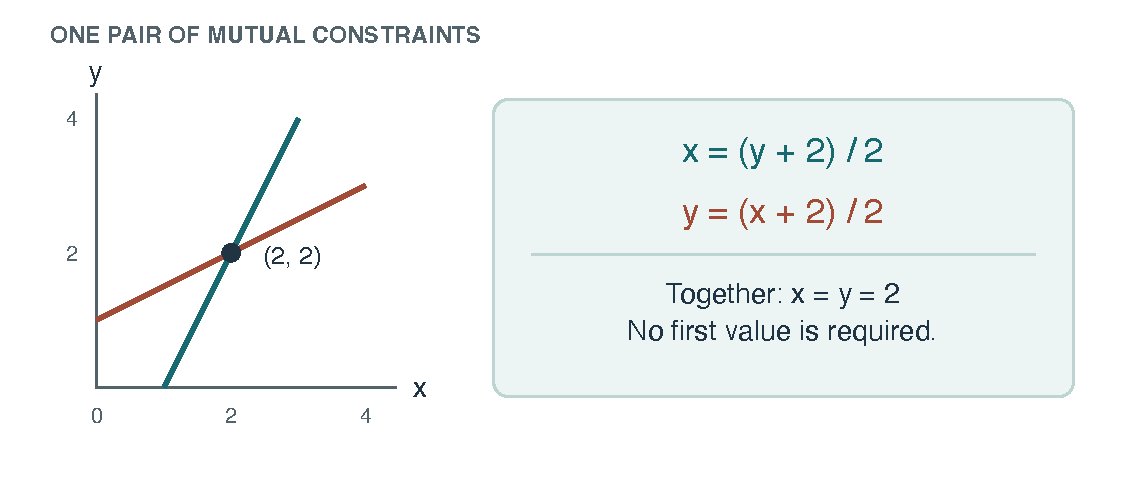
\includegraphics[keepaspectratio,alt={Mutual constraint can determine two values without giving either causal priority. The equations have one solution; equality alone would leave infinitely many.}]{figures/fig-mutual-constraint.pdf}}
\caption{Mutual constraint can determine two values without giving
either causal priority. The equations have one solution; equality alone
would leave infinitely many.}
\end{figure}

There is an immediate objection. Somebody selected those equations. Why
those?

Exactly. A fixed point earns an explanation relative to a map. It does
not explain the map merely by having one. Moving an unexplained choice
from a constant into an equation leaves the debt unpaid. A useful
account must identify the inputs it assumes, show the restrictions they
impose, and avoid hiding the desired answer in those inputs.

The example nevertheless establishes something consequential.
Determination need not proceed down a chain with a first term. The
picture of explanation as a row of falling dominoes is too narrow even
for two numbers.

\subsection{4. A world built from
comparisons}\label{a-world-built-from-comparisons}

The proposed architecture begins with bounded systems. Each has local
state, interfaces through which it encounters neighbours, and records
that later updates can consult. An observer, in this technical sense,
can be a measuring device or a software process. Consciousness is a
separate question.

These are substantive starting assumptions. The absence of an outside
observer does not prove that the world is finite, that its parts are
local, or that no common clock exists. They let us ask what a world must
be like if access to it is always situated within it.

Two observers need not contain identical records. One may describe a
shared edge in centimetres and another in millimetres. Agreement
requires a translation that makes their shared claims compatible.

Call a permitted revision a repair. For a finite model, let the total
discrepancy be

\[
  \Phi(s)=\sum_{e=\{u,v\}}w_e\,
  d_e\bigl(\pi_{u,e}(s_u),\pi_{v,e}(s_v)\bigr).
\]

Here \(s_u\) is one observer's state, \(\pi_{u,e}\) is its readout on a
shared interface, and \(d_e\) compares the two readouts in agreed terms.
The weights are fixed and nonnegative. An observer revises only its own
state, preserving protected evidence, and accepts a move only if the sum
on its incident edges strictly falls.

Untouched edges stay unchanged, so the global sum falls by precisely the
change on the touched edges. An observer can contribute to a global
improvement without representing the global quantity. The mathematician
uses the sum to prove something about the system; the system needs no
mathematician consulting it.

An outside description of a process can be global even when nothing
inside the process has global access. Requiring a coordinator because
our proof mentions a total would confuse how we understand the mechanism
with how the mechanism operates.

On a finite graph with finite effective state spaces, strict descent
permits only finitely many accepted repairs. It does not guarantee that
the last state satisfies every constraint. Nor does it guarantee that
different choices of repair end together. Those are separate demands:
enough repairs to reach consistency, and compatibility among alternative
repair paths.

When termination and local confluence hold, Newman's (1942) lemma
supplies confluence: branches from the same starting state can rejoin.
Determination by evidence requires more. Distinct starting states
carrying the same protected evidence must also have the same consistent
public output. A private bit untouched by every repair would otherwise
preserve a difference forever.

An objective answer needs to survive differences in how it is reached,
and the evidence must determine the answer being claimed. Order
independence alone cannot turn incomplete evidence into knowledge.

\subsection{5. Inconsistency without an
owner}\label{inconsistency-without-an-owner}

Give three observers a binary register each, \(a,b,c\). Their interfaces
impose three requirements: \(a=b\), \(b=c\), and \(c\ne a\).

Any one interface can be satisfied. Any two can be satisfied together.
All three cannot: the first two force the opposite of the third.

The failure has no single owner. Each observer can point to a locally
reasonable requirement. Yet there is no world of these three bits in
which the complete specification holds. Repair may move the discrepancy
around; it cannot remove an inconsistency in what it has been asked to
satisfy.

Change the third requirement to \(c=a\). There are two labelled
solutions, \(000\) and \(111\). If flipping all bits merely changes
notation, they describe one public state. If their labels have
observational meaning, two possibilities remain. Protect \(a=0\) as
evidence and only \(000\) survives.

Consistency excludes impossible candidates. Evidence can remove
alternatives. Neither operation, by itself, proves physical
instantiation.

\subsection{6. Computation, clocks, and
change}\label{computation-clocks-and-change}

A program encourages a sequential picture: provide an input, execute
instructions, obtain an output. Constraint computation separates the
relation defining the answer from the procedure finding it.

Take a register relation \(z=x\mathbin{\mathrm{XOR}}y\), where the
output is one exactly when the inputs differ. Fix \(x\) and \(y\) and it
computes \(z\). Fix \(x\) and \(z\) and the same relation determines
\(y\). Fix only \(z=1\) and it leaves two possible pairs. Ask for
\(x=y\) while protecting \(z=1\) and it reports an obstruction.

The relation has no intrinsic input end. The question acquires a
direction from what the questioner holds fixed.

Local records and repairs can implement these constraints, provided
permitted moves reach compatible states and preserve protected data. A
solver's sequence specifies order; a physical clock can additionally
measure the duration of its execution.

The word ``time'' needs the same care. Temporal order concerns which
events precede which; physical duration adds how much time elapses along
a path. A clock is a system furnishing readings. Its readings measure
duration only through a justified calibration. Neither kind of time is
the closure equation itself.

Five quantities must be kept apart. A repair index is a position in a
solver's sequence; different schedules can take different numbers of
steps to the same result. A logical clock numbers events respecting
causal precedence and supplies no seconds. A physical clock is a process
with countable changes, calibrated to measure proper time along its
path. A time coordinate labels events in a description and is no clock.
A simulator's host clock and the model's internal clock readings need
not agree in rate.

Order alone fixes no duration: multiplying every logical reading by ten
preserves precedence.\footnote{Lamport's (1978) logical clocks make this
  separation precise.} Likewise, a slower simulator can preserve all
internal clock comparisons if it preserves the model's complete
dynamics. A repair counter cannot silently substitute for either clock.

Timelessness means that the complete dependency structure needs no
external time to become a history. It does not remove the history's
internal changes. An observer's clock is one process within that
history.

A fundamental time could order events; that would not itself explain why
the ordered world exists. Requiring an earlier activation of time would
merely repeat the question. Closure avoids that requirement. This is its
explanatory advantage, without a proof that every theory with
fundamental time is inconsistent.

A result can then become a record that constrains another computation,
so that the system uses a description through its own activity. An
explanation of everything must include systems that use explanations.

\subsection{7. The closure condition}\label{the-closure-condition}

Let \(\mathfrak U\) denote a candidate inhabited structure. Let
\(D(\mathfrak U)\) denote an account of its architecture recoverable
through records within it. Let \(R\) denote an admissible realization of
that account. The closure condition is

\[
  R\bigl(D(\mathfrak U)\bigr)\ \cong\ \mathfrak U.
\]

The symbol \(\cong\) means agreement in the relevant observable and
interventional structure. The observations used to recover the
description, and the effects of actions available within the
realization, must fit the world from which the account was recovered.

The equation does not picture an external computer making a smaller
universe inside a larger one. Here realization means that the specified
state dependencies actually obtain, including their responses to
admitted interventions. It identifies the construction-side and
inhabited-side readings as readings of one system. This identification
is the closure hypothesis.

A recorded film can reproduce an experiment's outcomes along one
history. It cannot reproduce the experiment if changing the apparatus
leaves the film unchanged. A faithful realization must preserve the
dependencies through which a question can enter and a consequence can be
checked.

Nor does one finite observer have to contain a lossless copy of
everything. Records and models can be distributed, and an architecture
can be specified without enumerating every state it permits.

Self-reference earns nothing unless the return condition restricts the
possibilities. On the real numbers, \(T(x)=x+1\) has no fixed point,
\(T(x)=x\) has every point fixed, and \(T(x)=(x+2)/2\) has exactly one.
Writing \(x=T(x)\) is the beginning of a question.

\begin{figure}
\centering
\pandocbounded{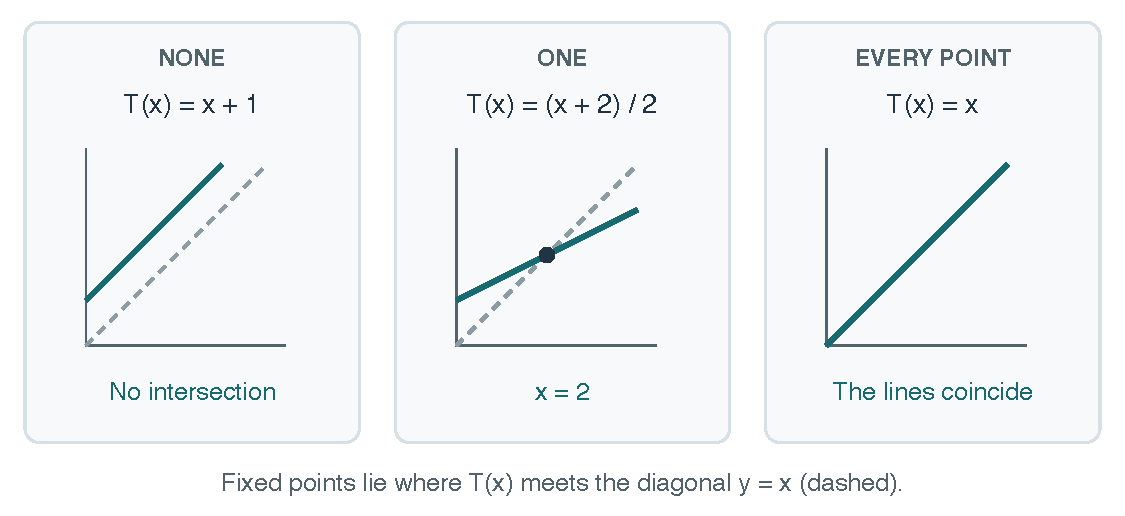
\includegraphics[keepaspectratio,alt={The same fixed-point notation admits no solution, every solution, or one solution. The explanatory work belongs to the specified map and its constraints.}]{figures/fig-closure-tests.pdf}}
\caption{The same fixed-point notation admits no solution, every
solution, or one solution. The explanatory work belongs to the specified
map and its constraints.}
\end{figure}

Lawvere's (1969) theorem gives a general account of certain diagonal
fixed-point constructions under a representation hypothesis.
Unrestricted self-representation fails in ordinary sets with nontrivial
outputs, by Cantor's argument. Useful restricted settings must justify
their admissible maps and closure properties. It would be a mistake to
infer a universe from the mere presence of self-reading.

What the equation supplies here is the form of a proposed explanation.
The candidate has to return its own world when its internally
recoverable description is realized. Its observations cannot demand one
architecture while its realization supplies another.

Nozick (1981) proposed that a fundamental principle might be
self-subsuming, explaining its own holding as one of its instances. The
closure condition is a self-subsuming requirement of that kind, with a
further demand: the subsumption must be inhabited, carried out through
records and agents inside the structure rather than stated about it from
outside.

The question is therefore inside the answer in a specific way. The
records that pose the reconstruction problem, the agents doing the
reconstruction, and the activity that realizes it are constituents of
the object being reconstructed. We have removed the external questioner
without removing the question.

\subsection{8. The meaning of ``nothing''}\label{the-meaning-of-nothing}

A closure account seeks laws that follow from relations which must fit
together. A quantity recovered independently from two descriptions of
the same interface cannot take incompatible values. Their agreement may
remove an apparent free parameter. The question changes from ``who set
this dial?'' to ``was there an independent dial?''

The architecture and both physical identifications still need
justification. An equation adjusted to a known answer merely encodes it,
and a unique solution within one architecture need not exclude every
other architecture.

Could the starting point be ``nothing'': a perfectly symmetric state, or
a uniformly random computation?

Those suggestions describe different conditions. \textbf{Absolute
absence} supplies no states, law, machine, or probability measure. A
computation supplies all the structure needed to count as that
computation, even when its output says ``nothing.'' A blank tape exists;
the emptiness it represents does not turn into an object by being
represented.

\textbf{Perfect symmetry} means invariance under specified
transformations. It need not mean absence of relations. Two unlabelled
positions can stand in a definite relation without either being
privileged. Only if every admissible state is observationally equivalent
is there just one distinguishable public possibility.

\textbf{Uniform randomness} leaves an outcome unspecified, given a
stated set of alternatives. For \(N\) equally likely alternatives,
Shannon's (1948) entropy is \(H=\log_2N\), its maximum. A simple rule
can specify that distribution without specifying its sampled outcome.
Simplicity of the rule, uncertainty about the outcome, and absence of
existence are three different things.

Here is the useful surprise. Let two bits have joint probabilities

\[
 P(0,0)=P(1,1)=\tfrac12.
\]

Neither bit has a preferred value. Simultaneously exchanging zero and
one preserves the distribution. Yet their relation is definite: they
agree. An observer holding either bit can predict the other. The
symmetry survives while the relation carries information. Compare
independent fair bits: the individual distributions are identical, but
one tells us nothing about the other.

This makes a defensible sense of ``a nothing'': no preferred absolute
label, while comparisons support definite relative content. The shared
bit is a minimal correlation; it is no observer. Records, their causal
use, and the conditions for stable public agreement must still be
supplied.

No choice appears by algebraic magic. A deterministic rule that respects
a symmetry preserves a perfectly symmetric initial state: if \(gx=x\)
and \(T(gx)=gT(x)\), then \(gT(x)=T(x)\). An asymmetric outcome needs
asymmetry, nonunique solutions with a selection rule, or stochastic
selection. A symmetric distribution can have asymmetric individual
outcomes.

The proposed origin is therefore logical rather than an earlier event: a
world can have no privileged absolute description while possessing the
relations through which its parts distinguish anything at all. This does
not derive existence from absolute absence. It asks whether the demand
for something \emph{in addition to} the complete relational structure is
itself misplaced.

\subsection{9. Description and
realization}\label{description-and-realization}

A novel describes a person opening a door. The sentence exists; a person
need not open a door. Description alone therefore cannot be a sufficient
condition for the existence of its subject.

Mathematics supplies a sharper claim. Gödel's (1930) completeness
theorem for classical first-order logic says that a consistent theory
has a mathematical model. This concerns satisfaction of its sentences,
without guaranteeing the intended model, uniqueness, or a physical
world. Gödel's (1931) incompleteness results concern a different limit:
sufficiently strong, effectively axiomatized arithmetic cannot both
prove only truths and settle every sentence. An internally describable
world need not be one whose inhabitants can prove every truth about it.

The useful distinction is between representing a dependency and
realizing it. A sentence can say that a memory changes a decision. In a
self-reading system, an actual retained state must help determine the
continuation. The relevant connection must survive controlled changes to
that state. Merely writing ``because'' between two events supplies no
causal channel.

Consider a description with states \(x\in X\) and update rules \(T_a\),
where \(a\) specifies an allowed operation. A proposed realization has
actual states \(s\in S\), corresponding operations \(F_a\), and a fixed
readout \(p:S\to X\). Require the readout to cover the admitted
described states and satisfy

\[
 p\bigl(F_a(s)\bigr)=T_a\bigl(p(s)\bigr)
\]

for every admitted state and operation. Records and ports must have
identified counterparts. The operations include the relevant
interventions as well as the updates that occurred on one recorded run.
Their causal implementation must be established; choosing new labels
after each outcome cannot count as a fixed readout.

\noindent\begin{minipage}{\linewidth}

\textbf{Finite realization lemma.} If this condition holds for every
step, it holds for every finite admitted sequence:

\[
 p\bigl(F_{a_n}\cdots F_{a_1}(s)\bigr)
 =T_{a_n}\cdots T_{a_1}\bigl(p(s)\bigr).
\]

The proof is induction. The one-step condition moves \(p\) past the last
update; applying it repeatedly moves \(p\) past the whole sequence.
Consequently, a described difference between two intervention outcomes
must also appear in the realized readouts. The implementation carries
the tested causal organization, including what would happen under the
admitted alternatives.

\end{minipage}

A playback can fail this condition while matching every frame of one
history. Suppose a bit is meant to toggle. After zero, both a genuine
toggle and a recording can display one. Set the retained bit to one
instead. The toggle produces zero; a playback that ignores the
intervention still displays its predetermined one.

\begin{figure}
\centering
\pandocbounded{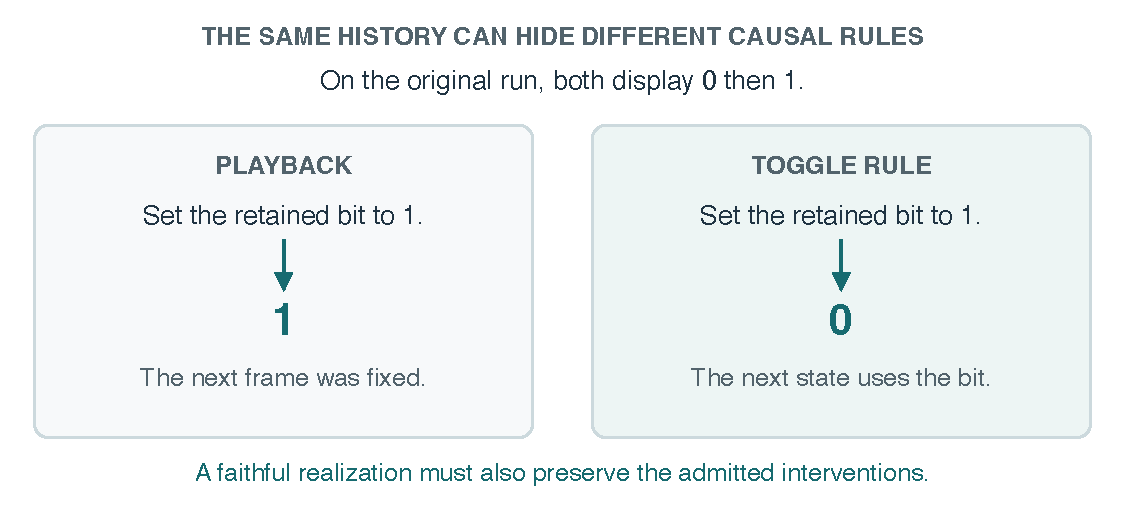
\includegraphics[keepaspectratio,alt={Matching one history does not establish the described causal rule. Changing the retained bit tests whether the next state depends on it. The difference concerns the specified state and intervention mapping.}]{figures/fig-description-and-realization.pdf}}
\caption{Matching one history does not establish the described causal
rule. Changing the retained bit tests whether the next state depends on
it. The difference concerns the specified state and intervention
mapping.}
\end{figure}

A printed transition table fails as a running implementation when its
entries do not govern corresponding state changes. Put it in a suitable
interpreter and the combined system may pass. Eligibility concerns the
organization supplied.

The ontological hypothesis can then be stated: \textbf{where a kind of
thing is constituted by a causal organization, a realization of that
organization is an instance of that kind.} The lemma checks fidelity;
the constitutive hypothesis says which properties that fidelity is
enough to instantiate. Chalmers's (2011) account of computational
implementation develops a related distinction between a formal
specification and its causal realization.

The qualification matters. A simulated flood can have actual
computational consequences without putting water on the host computer's
floor. A causal graph needs further geometric conditions to constitute a
spacetime. Consciousness requires the experiencing organization
specified by the phenomenal hypothesis, including its records,
self-reading, and ownership. A convincing display does not establish
those properties.

A physical simulator gives the lemma an actual implementing system. A
timeless universe raises the harder question: what realizes the entire
structure when there is no external machine?

The proposed answer is \textbf{intrinsic realization}: the complete
structure's lawful dependencies constitute its operation. States,
records, read/write relations, and responses to admissible variations
belong within it. A complete history contains change without needing a
further time in which that history is played. A record of that history
can be inert; the structure specified includes the dependencies through
which its inhabitants act.

Here is the ontological commitment: an inhabited, causally complete
closure is actual without an external act of actualization. The finite
lemma does not prove this, since it assumes an actual implementation.
The hypothesis extends the explanatory role of causal organization to
the totality, where borrowing an external implementing machine would
leave the original question unanswered. It is a restricted proposal in
the direction of Tegmark's (2008) mathematical-universe hypothesis,
focused on internally reconstructing observer worlds.

Why adopt it? Every test of existence available to an inhabitant is
already an encounter within the structure. Every clock tick, injury,
correction, and discovery has consequences there. An added stamp of
actuality would change none of those relations. The proposal identifies
reality with the complete organization responsible for them. A
philosopher can instead maintain that instantiation is an additional
primitive fact; the disagreement is ontological.

``Description is existence'' thus concerns the fully specified
qualifying structure, rather than the ink specifying it. Writing the
equation does not create the universe. On this hypothesis, its
inhabitants do not wait for us to write it. A novel that actually
specified such a complete structure would qualify; ordinary fiction
leaves that organization unsupplied.

This is the force of the mathematical insight: the structure need not
first exist as a possibility and then acquire a second property called
being switched on. Its internal operation constitutes its actuality. If
several closures qualify, the hypothesis admits several worlds;
predicting typical observations would require a justified measure.
Self-consistency alone has not selected our world.

\subsection{10. Made and found}\label{made-and-found}

Someone invents a game and then discovers a winning strategy they did
not invent. Choosing a rule and choosing its consequences are different
acts.

The strange loop takes this relation further. Its inhabitants can
recover the architecture of their world from its records and participate
in realizing that architecture through their activity. What is
discovered constrains what can be built. What is built is included in
the structure from which the discovery is made.

The usual dilemma demands that one side have absolute priority: either
the world exists fully before the knowers, who merely discover it, or
the knowers create the world. The dilemma borrows a chronological order
outside the total structure.

Inside the world, particular events have their ordinary order. Observers
gather evidence, infer rules, and construct something later. The closure
equation itself has no earlier stage at which one half has to wait for
the other. It specifies their mutual fidelity in a completed object.

Wheeler (1983) pictured a participatory universe as a self-excited
circuit, in which observers bring about the world that gives rise to
them. The closure condition keeps the circuit and removes the temporal
picture. Nothing observes before there is a world to observe; the loop
is a condition of mutual fidelity on the whole.

The pair of equations from section 3 showed the elementary form. We can
calculate \(x\) from \(y\) or \(y\) from \(x\). Neither calculation
makes the answer arbitrary. Neither demands that one quantity existed
first. The relations fix the pair together.

In the inhabited loop, the discovery is real because the consequences
resist preference. The construction is real because the agents' activity
is part of how the specified organization is realized. Knowing and
making are coupled roles within one world.

\begin{figure}
\centering
\pandocbounded{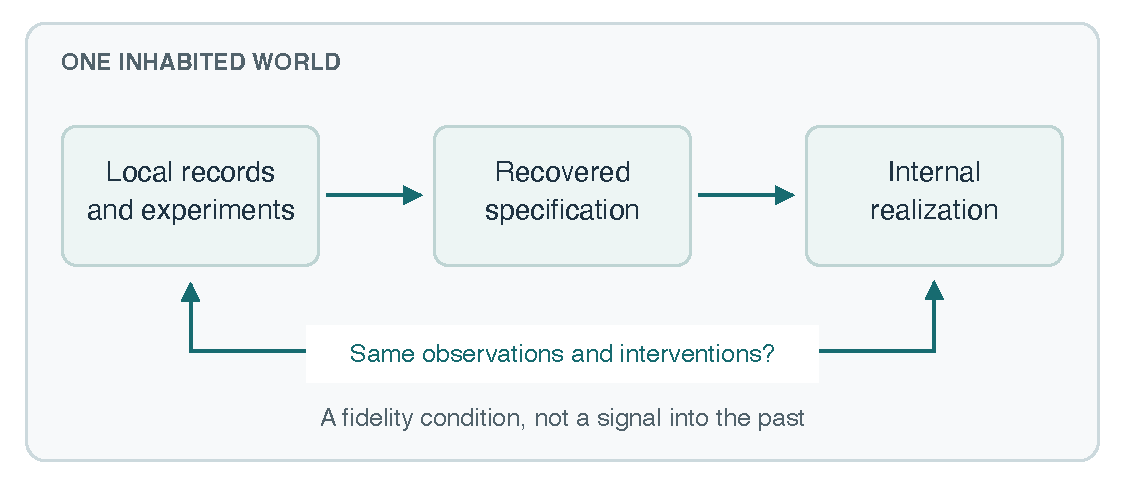
\includegraphics[keepaspectratio,alt={The closure hypothesis asks the inhabited world, an internally recovered specification, and its internal realization to agree on observations and interventions. The loop expresses mutual fidelity rather than a signal sent into the past.}]{figures/fig-inhabited-closure.pdf}}
\caption{The closure hypothesis asks the inhabited world, an internally
recovered specification, and its internal realization to agree on
observations and interventions. The loop expresses mutual fidelity
rather than a signal sent into the past.}
\end{figure}

What dissolves is the demand that discovery exclude participation. A
musician discovers what the score requires by playing it, and the
performance contributes something actual without choosing the musical
relations. In the loop proposed here, the score's own recovery and
realization belong to what is being performed.

The world is found in the constraints and made in their enactment. There
is no contradiction until one insists that a single verb must replace
both.

\subsection{11. Determination and
agency}\label{determination-and-agency}

The same mistake returns as a conflict between fate and freedom. If the
whole world is a fixed structure, what could an inhabitant possibly
decide?

Begin with the smaller theorem. Suppose a region has a unique consistent
public completion for each admitted boundary record \(b\). Write it as
\(N(b)\). An agent acts on the region by helping determine the record it
receives.

Uniqueness says that a specified input determines an answer. It does not
say that \(N(b)=N(b')\) for every pair of inputs. An agent who changes
the input can change the problem's solution. The inference from a
determined response to an irrelevant decision has silently removed the
decision from the arguments of the function.

An action can be determined through reasons and still make the
difference those reasons concern. The bridge responds to its load by
definite mechanics; deciding whether to place a load on it can remain
consequential. The mechanics carries the decision's effect.

Within a full history, there need not be another unfinished universe
waiting for us to fill in a blank. The act of deliberation is itself one
of the events constituting the history. Its consideration of
alternatives, sensitivity to evidence, and eventual commitment are how
this part of the answer gets determined.

This dissolves the competition between a complete structure and local
authorship. The structure is complete with the authorship in it. To
insist that it would have the same character without the authorship is
to propose a different dependency structure in place of explaining the
original one.

It does not settle every theory of free will. Someone requiring an
uncaused act will reject this account. The freedom defended here is a
situated capacity to represent alternatives, revise commitments for
reasons, and make interventions that change what follows. Those
capacities distinguish an agent from a passive conduit even when both
belong to a lawful world.

A person may be a small part of the world while being the place where
some consequential condition is set.

\subsection{12. The universe as a resolved
question}\label{the-universe-as-a-resolved-question}

A question normally seems distinct from its answer. ``What is the square
root of four?'' is a sentence; two is a number.

Constraint computation revealed another relation. A question specifies
what must fit. An answer is a state in which it fits. In a physical
implementation, the question is embodied in the constraints, and
answering is the activity of finding or realizing a compatible state.

Apply that form to the closure proposal. What is a universe like whose
records disclose an architecture that its own activity consistently
realizes? The unknown includes the records, the recovering observers,
the architecture, and the realization. A satisfactory answer cannot
leave any of them outside.

The universe is then the self-answering question in this precise sense.
Its relations embody the conditions to be satisfied; its inhabited
structure is their satisfaction; and some of its parts can make that
relation explicit in a description that belongs to the same structure.

The question's physical form is the network of constraints. Its explicit
formulation arrives in the record history of an observer, who can
discover what the structure has been enacting without standing outside
it.

This is also why observers matter to the proposal beyond being creatures
we happen to like. A merely consistent abstract model need not contain
any account of itself. Inhabited self-reconstruction is a stronger
requirement. It asks for parts through which the world's organization
can become a usable description and through which that description can
enter its realization.

The extra requirement may exclude candidates that consistency alone
permits. It cannot be assumed to select exactly one, and its physical
implementation must be established. Its significance is that the world's
being intelligible from within has entered the account of what sort of
world it is.

We are accustomed to treating intelligibility as a happy accident: laws
happen to exist, and much later some beings happen to discover them. The
strange-loop hypothesis joins those facts. The capacities for recovery
and realization are among the relations that close the structure.

\newpage

\subsection{13. Conclusion: the margin of the
page}\label{conclusion-the-margin-of-the-page}

Return to the final explanation in your hands. The ink in the margin
belongs to its subject matter. So does the alteration in your
understanding, and so does the experiment you decide to build.

The explanation is being read by one of the processes it explains. That
reading can change what the process does. Where the account is realized,
the discovered structure becomes an effective condition of its own
further activity. Its being a description does not make the activity
less actual; its words matter through the relations they enter.

Discovery is the answer's resistance to arbitrary preference. Invention
is the activity through which parts of it acquire determinate form. The
whole structure includes the decisions; the decisions participate in
determining the whole structure. None of these roles requires a first
moment outside the world.

On the account defended here, this is why the question of existence has
the shape of a strange loop. A universe needs no external maker when its
realization and its internally recoverable account constitute one
inhabited closure. The unknown on both sides of the condition is the
same world.

No clock ticks outside the equation to make its world begin. The clocks,
beginnings, discoveries, and decisions are among the relations it
specifies. The mathematical insight becomes a claim about what
constitutes their reality: the complete inhabited structure is already
its own realization.

``What would a universe that consistently creates itself be like?'' The
answer includes the systems capable of asking, the constraints their
answers must respect, and the actions through which those constraints
are realized.

The universe is that question answered. And the reader who finally sees
the loop is one of the places where the answer has become able to state
its own question.

\subsection{References}\label{references}

Chalmers, David J. 2011. ``A Computational Foundation for the Study of
Cognition.'' \emph{Journal of Cognitive Science} 12: 325--359.

Gödel, Kurt. 1930. ``Die Vollständigkeit der Axiome des logischen
Funktionenkalküls.'' \emph{Monatshefte für Mathematik und Physik} 37:
349--360.

Gödel, Kurt. 1931. ``Über formal unentscheidbare Sätze der Principia
Mathematica und verwandter Systeme I.'' \emph{Monatshefte für Mathematik
und Physik} 38: 173--198.

Hofstadter, Douglas R. 1979. \emph{Gödel, Escher, Bach: An Eternal
Golden Braid}. New York: Basic Books.

Lamport, Leslie. 1978. ``Time, Clocks, and the Ordering of Events in a
Distributed System.'' \emph{Communications of the ACM} 21: 558--565.

Lawvere, F. William. 1969. ``Diagonal Arguments and Cartesian Closed
Categories.'' \emph{Lecture Notes in Mathematics} 92: 134--145.

Leibniz, G. W. 1714. \emph{Principes de la nature et de la grâce fondés
en raison}. In \emph{Philosophical Essays}, translated by R. Ariew and
D. Garber. Indianapolis: Hackett, 1989.

Mueller, Bernhard, Alexander Osika, Mario Poneder, Kai Xue, Ben Cassie, Peter
Nguyen, Jinwook Kim, David Matscheko, Jonathan Hill, William T. Glynn, Maarten
Antonie Visser, Kale Arnav Anirudha, and Brieuc de La Fournière. 2026. ``Finite
Observer Consensus as a Reconstruction Principle: Normal Forms, the Standard
Model Lie Type, and a Route to the Einstein Field Equation.'' PhilPapers record
MUEFOC. \url{https://philpapers.org/rec/MUEFOC}.

Newman, M. H. A. 1942. ``On Theories with a Combinatorial Definition of
`Equivalence'.'' \emph{Annals of Mathematics} 43: 223--243.

Nozick, Robert. 1981. \emph{Philosophical Explanations}. Cambridge, MA:
Harvard University Press.

Parfit, Derek. 1998. ``Why Anything? Why This?'' \emph{London Review of
Books} 20 (2): 24--27; 20 (3): 22--25.

Shannon, Claude E. 1948. ``A Mathematical Theory of Communication.''
\emph{Bell System Technical Journal} 27: 379--423.

Tegmark, Max. 2008. ``The Mathematical Universe.'' \emph{Foundations of
Physics} 38: 101--150.

Wheeler, John Archibald. 1983. ``Law without Law.'' In \emph{Quantum
Theory and Measurement}, edited by J. A. Wheeler and W. H. Zurek,
182--213. Princeton: Princeton University Press.

\end{document}
